%% ------------------------------------------------------------------------- %%
\chapter{Contexto Teórico}
\label{cap:conceitos}

Este capítulo apresenta, um a um, os conceitos mais elementares, 
e tenta harmonizar a terminologia empregada no decorrer do texto.


%% ------------------------------------------------------------------------- %%
\section{\Gls{tectonic}}
\index{\gls{tectonic}}
\label{sec:02_tectonica}

A \gls{tectonic} é um \glsdesc*{tectonic}.

Uma das principais evidências das transformações geológicas do planeta 
são os \glspl{equake}. A figura \ref{f:global_epicenters} \citep{img_world_epicenters}
é um mapa global com a ocorrência geográfica dos tremores. Nele é possivel notar que 
os sismos não são distribuídos uniformemente pelo globo.

\begin{figure}[!h]
   \centering
   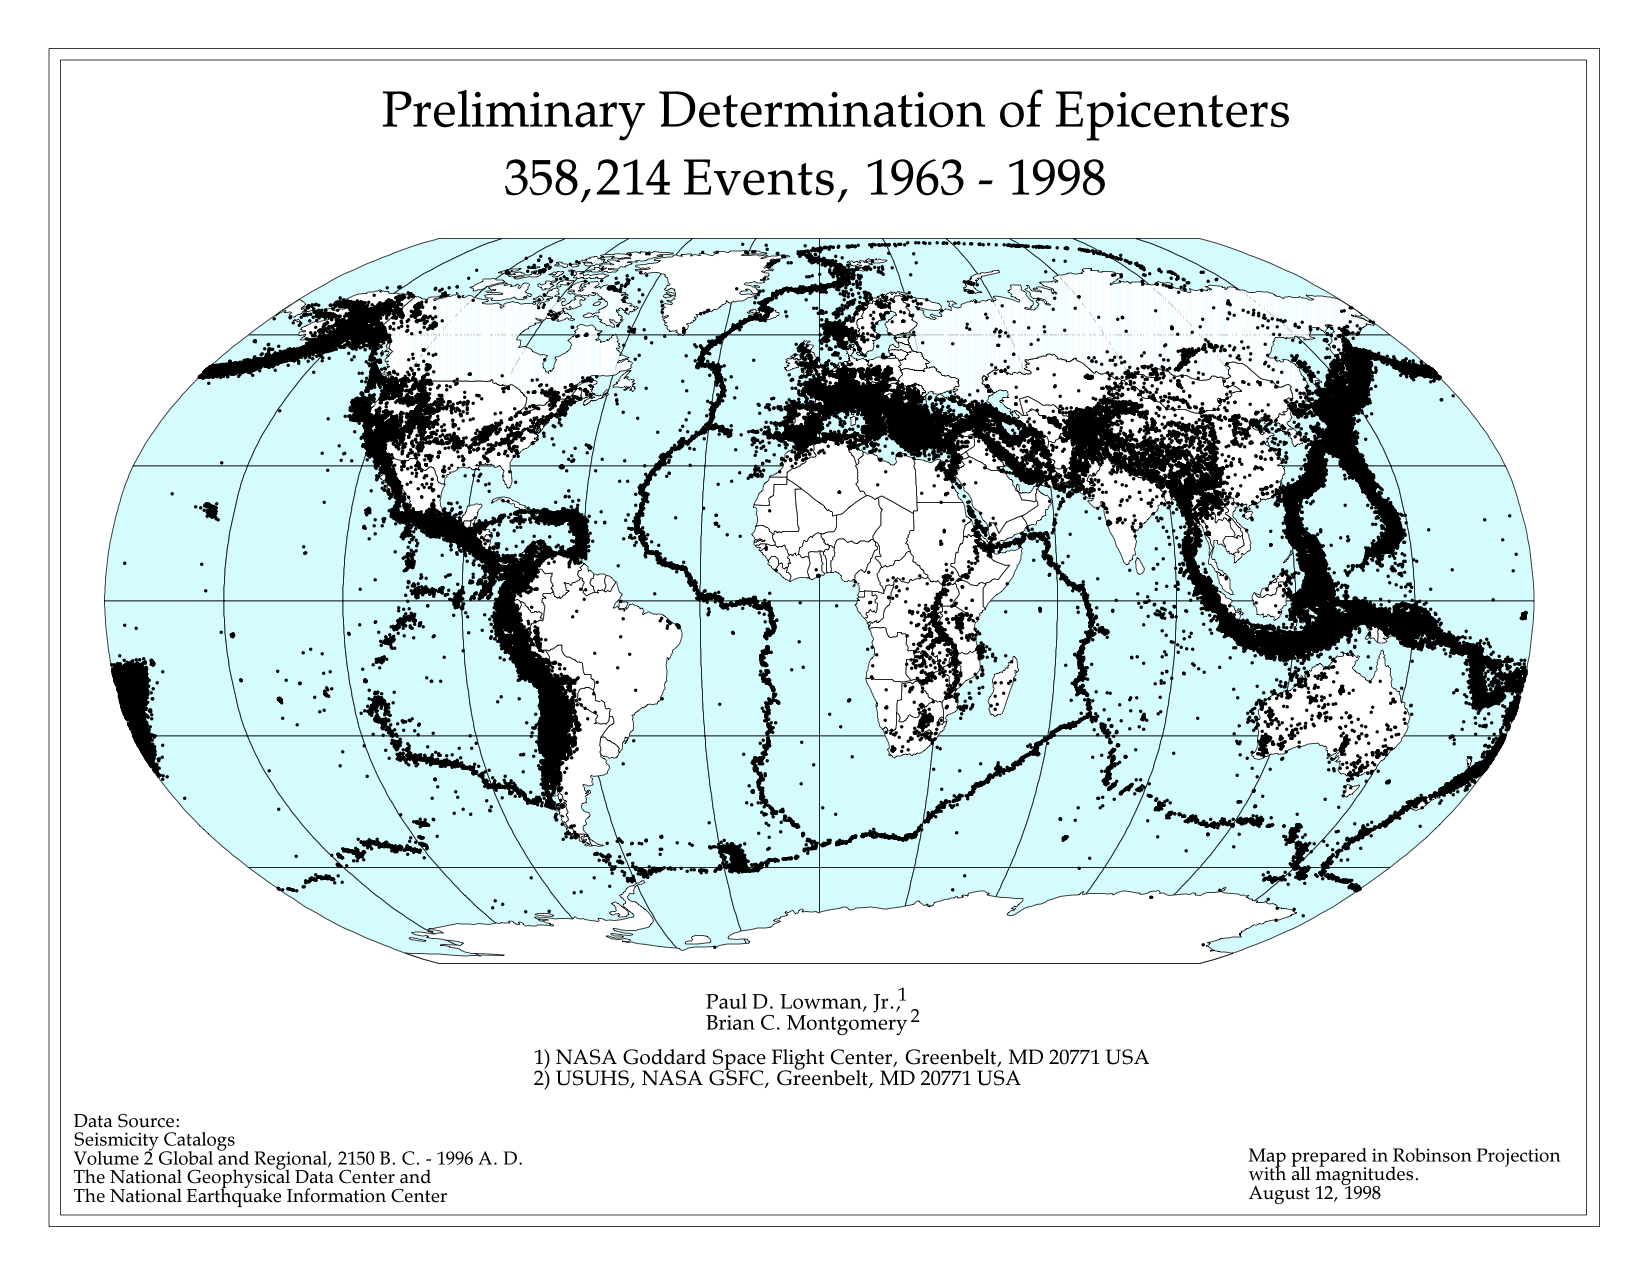
\includegraphics[width=0.80\textwidth]{global_pde_mag_all}
   \caption[Mapa Mundial de Epicentros 1963-1998]
   		   {Mapa Mundial de Epicentros 1963-1998\footnotemark} 
   \label{f:global_epicenters}
\end{figure} 
\footnotetext{\citet{img_world_epicenters}}
 
O padrão apresentado pela \gls{seismic_activity} global foi essencial 
para o desenvolvimento posterior da \gls*{tectonic_plate_theory}.

%% ------------------------------------------------------------------------- %%
\subsection{\Gls{tectonic_plate_theory}}
\index{\Gls{tectonic}!\Gls{tectonic_plate_theory}}
\label{sec:02_placas}

A \gls*{tectonic_plate_theory}, desenvolvida na segunda metade do século XX,
cartografava na superfície do globo as \glspl{litho_plate}.


\begin{figure}[!h]
   \centering
   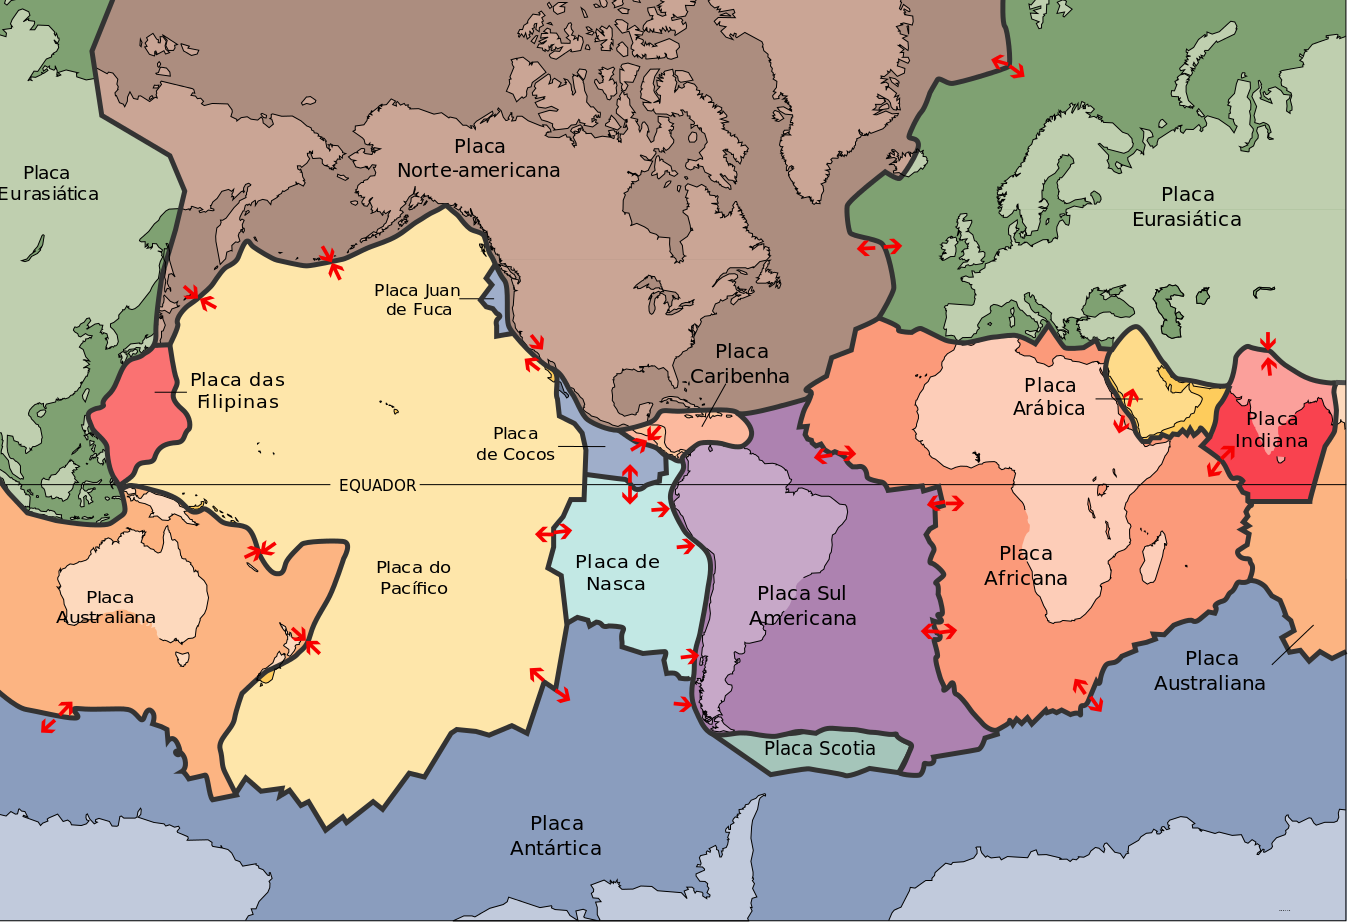
\includegraphics[width=0.80\textwidth]{litho_plates_overview}
   \caption[Cartografia das placas litosféricas]
   		   {Cartografia das placas litosféricas\footnotemark} 
   \label{f:plates_overview}
\end{figure} 
\footnotetext{\citet{img_plates_overview}}
 

As \glspl{litho_plate}, como pode ser visto na figura \ref{f:plates_overview} 
e o conceito de \gls{astenosphere} (\glsdesc{astenosphere}) 
surgem para conformar uma teoria capaz de explicar
uma série de fenômenos tectônicos já observados e ainda não bem explicados na época
de seu desenvolvimento. 


%% ------------------------------------------------------------------------- %%
\subsubsection{Bordas}
\index{\Gls{tectonic_plate_theory}!bordas}
\label{sec:02_bordas}

Nas bordas das \glspl{litho_plate}, a tectônica é mais intensa, 
provocando uma enorme diversidade de fenômenos geológicos de acordo
com o tipo de interação, como ilustrado na figura \ref{f:plate_boundaries}.

\begin{figure}[!h]
   \centering
   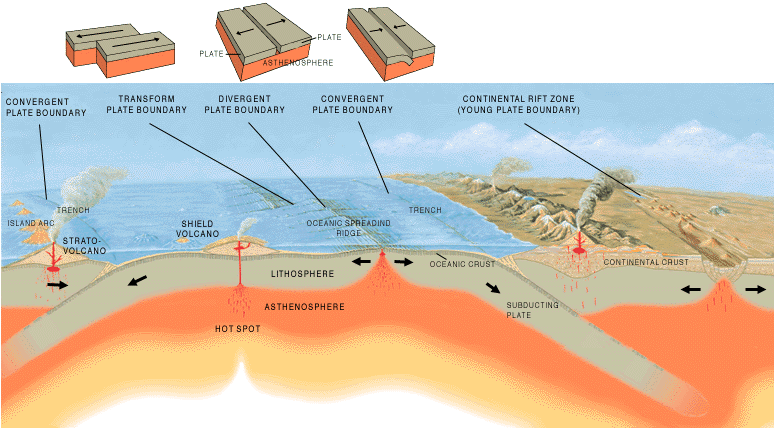
\includegraphics[width=0.80\textwidth]{plate_boundaries}
   \caption[Diferentes tipos de interações entre \glspl{litho_plate} em suas bordas]
   		   {Diferentes tipos de interações entre \glspl{litho_plate} em suas bordas\footnotemark} 
   \label{f:plate_boundaries}
\end{figure} 
\footnotetext{\citet{img_plate_boundaries}}
 
Na figura \ref{f:plate_boundaries} estão ilustrados os diferentes tipos de interação 
entre as \glspl{litho_plate} nas suas bordas, que causam, como já se sabe, a maior
parte dos \glspl{equake} e vulcanismo.

Só na borda das placas é liberada cerca de 95\% da quantidade total da energia 
liberada em \glspl{equake} no globo.


%% ------------------------------------------------------------------------- %%
\subsubsection{Interior}
\index{\Gls{tectonic_plate_theory}!interior}
\label{sec:02_interior}

A dificuldade maior é explicar, com maior detalhe, porque e como são liberados os outros 
5\% do total de energia nos \glspl{equake}, mais raros, no interior das \glspl{litho_plate}.

Não há pleno consenso nem um modelo geral para a explicação do mecanismo de ocorrência dos
sismos no interior das placas, embora sejam conhecidas diversas zonas sísmicas em regiões no interior
de placas, como em Nova Madrid, nos Estados Unidos e também em locais da China e da Austrália para citar alguns.


%% ------------------------------------------------------------------------- %%
\subsection{Sismotectônica}
\index{\gls{tectonic}!\gls{seismotectonic}}
\label{sec:sismotectonica}

A \gls{seismotectonic} é \glsdesc*{seismotectonic}. 

Na prática consiste por um lado, num esforço de compreensão dos
processos geológicos através da observação dos tremores e analogamente, compreender os tremores através da observação
de processos geológicos mensuráveis.  

É fácil notar, portanto, a contribuição dessa disciplina na análise da sismicidade.


\section{Sismicidade}
\index{sismicidade}
\label{sec:sismicidade}

A sismicidade é o estudo da frequência de ocorrência de tremores de terra, no
tempo e no espaço.

Tremores de terra, abalos, \glspl{equake}, sismos são a ocorrência de
fenômenos geológicos de ruptura 'instanânea', com um certo tamanho, na
crosta terrestre.


\subsection{Ocorrência}
\index{\gls{equake}!ocorrência}
\label{sec:ocorrencia}
 
A ocorr{\^e}ncia dos tremores se d{\'a} num tempo {$t$} e num lugar {$r$} da
crosta que pode ser considerado simplificadamente ora como
bi-dimensional: o eapaço dos \emph{epicentros} $ E = {(x,y)}$, ora como
tri-dimensional: o espaço dos \emph{hipocentros} $ H = {(x,y,z)}$.

Na prática o que ocorre realmente é o deslocamento relativo (\emph{$rake$})
entre estruturas geologias em uma certa área \emph{$A_{rupture}$}, o falhamento geológico.


\subsubsection{Processo de Poisson}\index{área do
trabalho!fundamentos}
\label{sec:risco_sismico}

Definição do processo\ldots

Críticas\ldots


\subsubsection{Independência entre eventos}\index{área do
trabalho!fundamentos}
\label{sec:risco_sismico}

Pressupostos\ldots

Críticas\ldots


\subsubsection{Omori-Utsu}\index{área do
trabalho!fundamentos}
\label{sec:risco_sismico}

Definição do processo\ldots

Críticas\ldots


\subsection{Falhamento Geológico}
\index{área do trabalho!fundamentos}
\label{sec:risco_sismico}

De forma simplificada, os falhamentos geológicos podem ser classificados em três
grupos segundo a teoria da tecônica de placas, que versa sobre a interação
entre crosta e o manto terrestre e seus reflexos na geologia crustal:

\subsubsection{Falhamento Normal}\index{área do
trabalho!fundamentos}
\label{sec:risco_sismico}

Ou seja que ocorrem em regime de compressão


\subsubsection{Falhamento Reverso}\index{área do
trabalho!fundamentos}
\label{sec:risco_sismico}

Ou seja, por distenção, fenômeno mais raro como a abertura de oceanos 


\subsubsection{Falhamento Transcorrente/Transverso}\index{área do
trabalho!fundamentos}
\label{sec:risco_sismico}

O que ocorre de maneira oblíqua, em regimes de cisalhamento.



 
\subsection{Predição da Ocorrência de Rupturas}\index{área do
trabalho!fundamentos}
\label{sec:fundamentos}

Texto texto texto texto texto texto texto texto texto texto texto texto texto
texto texto texto texto texto texto texto texto texto texto texto texto texto
texto texto texto texto texto texto texto texto texto texto texto texto texto


\subsubsection{Curto-prazo}\index{área do trabalho!fundamentos}
\label{sec:fundamentos}


Texto texto texto texto texto texto texto texto texto texto texto texto texto
texto texto texto texto texto texto texto texto texto texto texto texto texto
texto texto texto texto texto texto texto texto texto texto texto texto texto


\subsubsection{Longo-prazo}\index{área do trabalho!fundamentos}
\label{sec:fundamentos}

Texto texto texto texto texto texto texto texto texto texto texto texto texto
texto texto texto texto texto texto texto texto texto texto texto texto texto
texto texto texto texto texto texto texto texto texto texto texto texto texto
texto texto texto texto texto texto texto texto texto texto texto texto texto
texto texto texto texto texto texto.


 
\subsection{Magnitude - Tamanho da Ruptura}\index{área do
trabalho!fundamentos}
\label{sec:risco_sismico}

A magnitude de um tremor de terra, é um valor medido numa escala que busca
refletir a energia liberada pelo tremor de terra como sendo proporcional à área
e ao deslocamento da ruptura geológica que o originou.

O desenvolvimento das escalas de magnitude para medir o tamanho dos tremores,
iniciou-se experimentalmente com Richter e segue até sua corrente definição



\subsubsection{Magnitude Richter }\index{área do
trabalho!fundamentos}
\label{sec:risco_sismico}

O desenvolvimento das escalas de magnitude para medir o tamanho dos tremores,
iniciou-se experimentalmente com Richter e segue até sua corrente definição


\subsubsection{Magnitude de Momento Sísmico }\index{área do
trabalho!fundamentos}
\label{sec:risco_sismico}

O desenvolvimento das escalas de magnitude para medir o tamanho dos tremores,
iniciou-se experimentalmente com Richter e segue até sua corrente definição





\subsubsection{Intensidade Macrossísmica}
\index{área do trabalho!fundamentos}
\label{sec:risco_sismico}


A intensidade macrossísmica é uma escala para medir, não a energia proporcional
à ruptura que originou o tremor de terra, mas para retratar a percepção do
movimento do chão onde quer tenha produzido seus efeitos perceptíveis ao ser
humano.

Uma das mais difundidas é a escala de Mercalli:


TABELA


Existem estudos que propõem a inferência sobre o tamanho da ruptura, e sua
magnitude, a partir de observações macrossísmicas, ou relatos georreferenciados.






%% ------------------------------------------------------------------------- %%
\subsection{Representação}\index{área do trabalho!fundamentos}
\label{sec:fundamentos}


%% ------------------------------------------------------------------------- %%
\subsubsection{Epicentros}\index{área do trabalho!fundamentos}
\label{sec:fundamentos}

Epicentros $ E : {(x,y,t,m)}$

Com incertezas

$ E : {(x,\sigma_x,y,\sigma_y,t,\sigma_t,m,\sigma_m)}$


%% ------------------------------------------------------------------------- %%
\subsubsection{Hipocentros}\index{área do trabalho!fundamentos}
\label{sec:fundamentos}

hipocentros $ H : {(x,y,z,t,m)}$

Com incertezas

hipocentros $ H : {(x,\sigma_x,y,\sigma_y,z,\sigma_z,t,\sigma_t,m,\sigma_m)}$


%% ------------------------------------------------------------------------- %%
\subsubsection{Falhamentos}\index{área do trabalho!fundamentos}
\label{sec:fundamentos}

Falhamentos ocorrem como deslocamentos em planos 

$ F : {(d,s,r)}$

Dip, Strike, Rake



%% ------------------------------------------------------------------------- %%
\subsubsection{Rupturas}\index{área do trabalho!fundamentos}
\label{sec:fundamentos}

Falhamentos ocorrem como deslocamentos como tensores 

$ F : {(d,s,r)}$




\subsection{Distribuição de Frequência e Magnitudes}\index{área do
trabalho!fundamentos}
\label{sec:risco_sismico}

À uma primeira abordagem estatística, seria conveniente analisar a frequência de
ocorrencia dos sismos.

\subsubsection{Gutemberg-Richter MFD}\index{área do
trabalho!fundamentos}
\label{sec:risco_sismico}

Gutemberg e Richter, por terem desenvolvido à escala de tamanho dos
tremores, foram os primeiros a analisar sua frequência de ocorrencia com estes
mesmos tamanhos.

A observação de que a forma da sua distribuição se caracterizava por uma 
XXXXX, é utilizada até hoje para a estimativa da ocorrencia de tremores futuros.



\subsubsection{Truncated MFD}\index{área do
trabalho!fundamentos}
\label{sec:risco_sismico}

Como variações ou critérios de contorno, algumas distribuições foram surgindo,
como por exemplo a distribuição truncada de magnitude e frequência (TMFD):


FORMULAS


GRAFICO



\subsubsection{Tapered MFD}\index{área do
trabalho!fundamentos}
\label{sec:risco_sismico}


Existe também distribuições que terminam suavemente em magnitudes menos
elevadas, sugerindo a raridade dos fenomenos geológicos ou o tempo escasso de
observação.


\subsubsection{Exponential cutoff MFD}\index{área do
trabalho!fundamentos}
\label{sec:risco_sismico}

Entretanto, fenômenos de maiores magnitudes podem ter sido noticiados em
maior quantidade sugerindo distribuições um pouco mais alongadas:

GRAFICO

FORMULA



\section{Taxa de Sismicidade}\index{área do
trabalho!fundamentos}
\label{sec:risco_sismico}


Texto texto texto texto texto texto texto texto texto texto texto texto texto
texto texto texto texto texto texto texto texto texto texto texto texto texto
texto texto texto texto texto texto texto texto texto texto texto texto texto


\subsubsection{Magnitude de Completude}\index{área do
trabalho!fundamentos}
\label{sec:risco_sismico}

A magnitude de completude\ldots 

texto texto texto texto texto texto texto texto texto texto texto texto texto


GRAFICO

FORMULA



\subsubsection{Valor-b}\index{área do
trabalho!fundamentos}
\label{sec:risco_sismico}


Texto texto texto texto texto texto texto texto texto texto texto texto texto
texto texto texto texto texto texto texto texto texto texto texto texto texto
texto texto texto texto texto texto texto texto texto texto texto texto texto


\subsubsection{Valor-a}\index{área do
trabalho!fundamentos}
\label{sec:risco_sismico}



Texto texto texto texto texto texto texto texto texto texto texto texto texto
texto texto texto texto texto texto texto texto texto texto texto texto texto
texto texto texto texto texto texto texto texto texto texto texto texto texto




\section{Risco Sísmico}\index{área do trabalho!fundamentos}
\label{sec:risco_sismico}

-> risk = ( hazard, 
			exposition, 
			vulnerability)


Texto texto texto texto texto texto texto texto texto texto texto texto texto
texto texto texto texto texto texto texto texto texto texto texto texto texto
texto texto texto texto texto texto texto texto texto texto texto texto texto



\section{Ameaça Sísmica}\index{área do trabalho!fundamentos}
\label{sec:ameaca_sismica}

-> hazard = seismic sources, 
			rupture occurence, 
			ground motion prediction 



Texto texto texto texto texto texto texto texto texto texto texto texto texto
texto texto texto texto texto texto texto texto texto texto texto texto texto
texto texto texto texto texto texto texto texto texto texto texto texto texto



\section{Análise Probabilistica de Ameaça Sísmica}\index{área do
trabalho!fundamentos}
\label{sec:psha}


cornell, mcguire ?!?


Texto texto texto texto texto texto texto texto texto texto texto texto texto
texto texto texto texto texto texto texto texto texto texto texto texto texto
texto texto texto texto texto texto texto texto texto texto texto texto texto



%% ------------------------------------------------------------------------- %%
\subsection{Caracterização de Fontes Sísmicas}
\index{ácido!nucléico}\index{nucleotídeos}
\label{sec:fontes}

cornell, mcguire ?!?


Texto texto texto texto texto texto texto texto texto texto texto texto texto
texto texto texto texto texto texto texto texto texto texto texto texto texto
texto texto texto texto texto texto texto texto texto texto texto texto texto



\subsubsection{Tipologia e Representação Geométrica}
\index{ácido!nucléico}\index{nucleotídeos}
\label{sec:fontes_tipologia}


\subsubsection{Falha Complexa}
\index{ácido!nucléico}\index{nucleotídeos}
\label{sec:fonte_falha_complexa}


Texto texto texto texto texto texto texto texto texto texto texto texto texto
texto texto texto texto texto texto texto texto texto texto texto texto texto
texto texto texto texto texto texto texto texto texto texto texto texto texto



\subsubsection{Falha Simples}
\index{ácido!nucléico}\index{nucleotídeos}
\label{sec:fonte_falha_complexa}



Texto texto texto texto texto texto texto texto texto texto texto texto texto
texto texto texto texto texto texto texto texto texto texto texto texto texto
texto texto texto texto texto texto texto texto texto texto texto texto texto



\subsubsection{Área}
\index{ácido!nucléico}\index{nucleotídeos}
\label{sec:fonte_falha_complexa}


Texto texto texto texto texto texto texto texto texto texto texto texto texto
texto texto texto texto texto texto texto texto texto texto texto texto texto
texto texto texto texto texto texto texto texto texto texto texto texto texto



\subsubsection{Pontos}
\index{ácido!nucléico}\index{nucleotídeos}
\label{sec:fonte_falha_complexa}


Texto texto texto texto texto texto texto texto texto texto texto texto texto
texto texto texto texto texto texto texto texto texto texto texto texto texto
texto texto texto texto texto texto texto texto texto texto texto texto texto



\subsection{Caracterização}
\index{ácido!nucléico}\index{nucleotídeos}
\label{sec:fontes}



Texto texto texto texto texto texto texto texto texto texto texto texto texto
texto texto texto texto texto texto texto texto texto texto texto texto texto
texto texto texto texto texto texto texto texto texto texto texto texto texto



\subsubsection{Ocorrência de Sismicidade}
\index{ácido!nucléico}\index{nucleotídeos}
\label{sec:fontes}


Texto texto texto texto texto texto texto texto texto texto texto texto texto
texto texto texto texto texto texto texto texto texto texto texto texto texto
texto texto texto texto texto texto texto texto texto texto texto texto texto


\subsubsection{Ocorrência de Sismicidade}
\index{ácido!nucléico}\index{nucleotídeos}
\label{sec:fontes}




Texto texto texto texto texto texto texto texto texto texto texto texto texto
texto texto texto texto texto texto texto texto texto texto texto texto texto
texto texto texto texto texto texto texto texto texto texto texto texto texto



\subsubsection{Caracterização de Fontes Sísmicas}
\index{ácido!nucléico}\index{nucleotídeos}
\label{sec:fontes}



Texto texto texto texto texto texto texto texto texto texto texto texto texto
texto texto texto texto texto texto texto texto texto texto texto texto texto
texto texto texto texto texto texto texto texto texto texto texto texto texto





%% ------------------------------------------------------------------------- %%
\subsection{Predição do Movimento do Chão} 
\index{ácido!nucléico}\index{nucleotídeos}
\label{sec:gmpe}


Texto texto texto texto texto texto texto texto texto texto texto texto texto
texto texto texto texto texto texto texto texto texto texto texto texto texto
texto texto texto texto texto texto texto texto texto texto texto texto texto

